\documentclass[11pt,a4paper,sans]{moderncv}        
%---------%---------%---------%---------%---------%---------%---------%---------
% Includes of packages, etc
%---------%---------%---------%---------%---------%---------%---------%---------
\moderncvstyle{banking}                            
\moderncvcolor{red}                               
\nopagenumbers{}
\usepackage[scale=0.75]{geometry}
\setlength{\footskip}{136.00005pt} 
\usepackage{titlesec}
\graphicspath{{../includes/}{../../images/}{../../photos/}}
\usepackage{enumitem}   
\usepackage[utf8]{inputenc}
\usepackage[T1]{fontenc}
\usepackage[svgnames]{xcolor}

\usepackage{helvet}  % Helvetica typsnitt
\newcommand{\customheading}[1]{%
  {\LARGE\bfseries\sffamily #1}%make
  \vspace{0.5em}%
  \par
}

\titleformat{\section}
  {\normalfont\Large\bfseries\sffamily} % Stil: fet, storlek, sans serif
  {\thesection}{1em}{} % Sektionens nummerformatering

\ifxetexorluatex{}
  \usepackage{fontspec}
  \usepackage{unicode-math}
  \defaultfontfeatures{Ligatures=TeX}
  \setmainfont{Latin Modern Roman}
  \setsansfont{Latin Modern Sans}
  \setmonofont{Latin Modern Mono}
  \setmathfont{Latin Modern Math} 
  \moderncvcolor{blue}    % ren, professionell
  % eller
  \moderncvcolor{burgundy}  % sofistikerad, djup röd
% eller
  \moderncvcolor{grey}      % elegant och diskret

\else
  \usepackage[utf8]{inputenc}
  \usepackage[T1]{fontenc}
  \usepackage{lmodern}
\fi

\usepackage[swedish]{babel}  
\usepackage{underscore} 
% ------- % ------- % ------- % ------- % ------- % ------- % -------
% ------- % ------- % ------- % ------- % ------- % ------- % -------
% Self-defined commands
% ------- % ------- % ------- % ------- % ------- % ------- % -------
% ------- % ------- % ------- % ------- % ------- % ------- % -------

%\newcommand{\thepage}{\arabic{page}}
\pagestyle{plain}  % eller 'empty', 'headings', 'fancy' m.m.
  
\newlist{quotelist}{enumerate}{1}
\setlist[quotelist]{label=\textquotedblleft\arabic*\textquotedblright}

\newcommand{\myparagraph}[1]{\paragraph{#1}\mbox{}\par}

\makeatletter

% Definiera bredden om den inte finns
\@ifundefined{@photowidth}{%
  \newlength{\@photowidth}
  \setlength{\@photowidth}{4cm} % Justera storleken här – t.ex. 3cm, 4cm, 5cm
}{}



% Modifiera \makecvtitle om stilen är 'banking'
\@ifpackageloaded{moderncvstylebanking}{%
  \let\oldmakecvtitle\makecvtitle
  \renewcommand*{\makecvtitle}{%
    \vspace*{-1em}
    \begin{center}
      \includegraphics[width=\@photowidth,keepaspectratio]{\@photo}
    \end{center}
    \vspace{0.5em}
    \oldmakecvtitle
  }%
}

\makeatother

    % ------ ---------- -------- ---------- ----------- ----------- ----------------
    % ------ ---------- -------- ---------- ----------- ----------- ----------------
    % 
    % Head Line : Role : Role
    %2-------- ----------------
    % ------ ---------- -------- ---------- ----------- ----------- ----------------
% {\Large \sffamily \bfseries IT-Support Engineer}\\[0.2em]

%\beforetitle{



%------------------%------------------%------------------%------------------%------------------
% Title - photo etc
%     {\color{gray}\large\sffamily JAVA\# } \\[1em]
%------------------%------------------%------------------%------------------%------------------       
\title{MSc, Software Engineering}      
%------------------%------------------%------------------%------------------%------------------ 
%------------------%------------------%------------------%------------------%------------------ 
\firstname{Rickard}
\lastname{\AA{}berg}
\address{Bodekullsgatan 34b}{21440 Malm\"o}
\phone[mobile]{+46~709~43~14~01}     
\email{rickard.aaberg@icloud.com}   
               

%------------------%------------------%------------------%------------------%------------------ 
% QUOTE
\quote{If you fall one-hundred times and then get up, the 101 time you never lost!}
%------------------%------------------%------------------%------------------%------------------

\begin{document}
%\makecvtitle{}
\begin{center}
    \vspace*{1cm}
    
    {\Huge \textbf{\textcolor{gray!20!black}{IT-Support Engineer}}}\\[1em]
    

    
\includegraphics[width=3.6cm]{../../photos/rickardaberg-consultant.jpeg} \\[1em]
    
    {\LARGE \textbf{Rickard Åberg}}\\[0.2em]
    {\large MSc in Software Engineering}\\[2em]
    
{\footnotesize
\begin{tabular}{l}
\texttt{Tel: +46 709 43 14 01} \\
\texttt{Email: rickard.aaberg@icloud.com} \\
\texttt{Location: Malmö, Sweden}
\end{tabular}
}
  
    \vspace*{1cm}
\end{center}
%}
\newpage

\renewcommand*{\namefont}{\LARGE\sffamily\mdseries}
\renewcommand*{\titlefont}{\Large\sffamily\mdseries}

% 💼 Professional Summary
% Resultatinriktad och serviceorienterad IT-tekniker med certifiering i Microsoft Azure (AZ-900) och över 10 års erfarenhet inom IT-support, systemutveckling och teknisk problemlösning. Pedagogiskt lagd och van vid att vägleda användare på alla nivåer – både tekniskt och kommunikativt – på svenska och engelska. Gedigen erfarenhet av både Windows, macOS och Linux, samt felsökning av nätverk, hårdvara, mjukvara och molnbaserade system. Brinner för att göra teknik begriplig och tillgänglig, och kombinerar teknisk kompetens med coachande förhållningssätt för att skapa trygghet, struktur och flyt i IT-miljöer.


% 💼 Professional Summary
% Driven och pedagogisk IT-supporttekniker med över ett decennium av erfarenhet inom teknisk problemlösning, användarstöd och systemintegration. Certifierad i Microsoft Azure (AZ-900) med bred kompetens inom Windows, macOS, Linux, nätverk och molntjänster. Van att kommunicera med både tekniska och icke-tekniska användare på svenska, engelska och franska. Brinner för att skapa trygghet i IT-miljöer genom strukturerat stöd, tydlig kommunikation och coachande bemötande.


\section{Professional Summary}

Har lång erfarenhet av \textbf{Application Management} och \textbf{Problem Management} i komplexa IT-miljöer, bland annat inom Telenor, Länsstyrelsen IT och Ikano Bank. \\
Har agerat länk mellan användarstöd, drift, utveckling och arkitektur, och har arbetat nära \textbf{Service Desk}, både operativt och strategiskt. \\
Har drivit \textbf{rotorsaksanalyser enligt ITIL}, förbättrat processer och implementerat lösningar som minskat antalet återkommande incidenter drastiskt. \\
Van att ta tekniskt ansvar för affärskritiska system, leda möten över flera team, och skapa struktur i både reaktiva och proaktiva IT-supportmiljöer.

\section{Industry Experience}

\cvitem{}{%
\textbf{Public Sector and Government:} Länsstyrelsen IT, Tre (Hi3G), SL (Stockholm Public Transit), IDA Infront \\
\textbf{Retail \& E-commerce:} IKEA IT, Ikano, Lindab \\
\textbf{Finance and Banking:} Nordea, Ikano Bank \\
\textbf{Telecom and Technology:} Telenor, Sony, Hi3G \\
\textbf{Healthcare and Biotech:} HemoCue, Verisure \\
\textbf{Education and Research:} École des Mines, ReDI School \\
\textbf{Aviation and Infrastructure:} ADB Safegate \\
\textbf{Hospitality and Lifestyle:} Hot Yoga Malmö, Radioforum \\
}



\cvitemwithcomment{French}{C1 – Advanced professional proficiency}{Used in project work with clients at École des Mines}

\section{Languages}
\cvitemwithcomment{Swedish}{Mother tongue}{}
\cvitemwithcomment{English}{Professional proficiency}{}
\cvitemwithcomment{French}{Professional proficiency}{}



\clearpage
\section{Certification Badges}
\cvitem{}{
  \begin{minipage}[t]{0.24\linewidth}
    \centering
    
\includegraphics[width=0.9\linewidth]{../../images/azure-fundamentals-badge.png}\\
    \scriptsize Microsoft Certified: Azure Fundamentals (AZ-900)
  \end{minipage}
  \hfill
  % \begin{minipage}[t]{0.24\linewidth}
  %   \centering
  %   \includegraphics[width=0.6\linewidth]{../../images/icc_coach.jpeg}\\
  %   \scriptsize ICC Certified Coach
  % \end{minipage}
  % \hfill
  \begin{minipage}[t]{0.24\linewidth}
    \centering
    
\includegraphics[width=0.6\linewidth]{../../images/ISQTB.jpg}\\
    \scriptsize ISTQB Certified Tester\\
    Foundation Level (CTFL)
  \end{minipage}
  \hfill
  \begin{minipage}[t]{0.24\linewidth}
    \centering
    
\includegraphics[width=0.9\linewidth]{../../images/Certified_Scrum_Master_(CSM)_certification_badge.PNG}\\
    \scriptsize Certified Scrum Master
  \end{minipage}
}

% \cvitem{}{
%   \begin{minipage}[t]{0.24\linewidth}
%     \centering
%     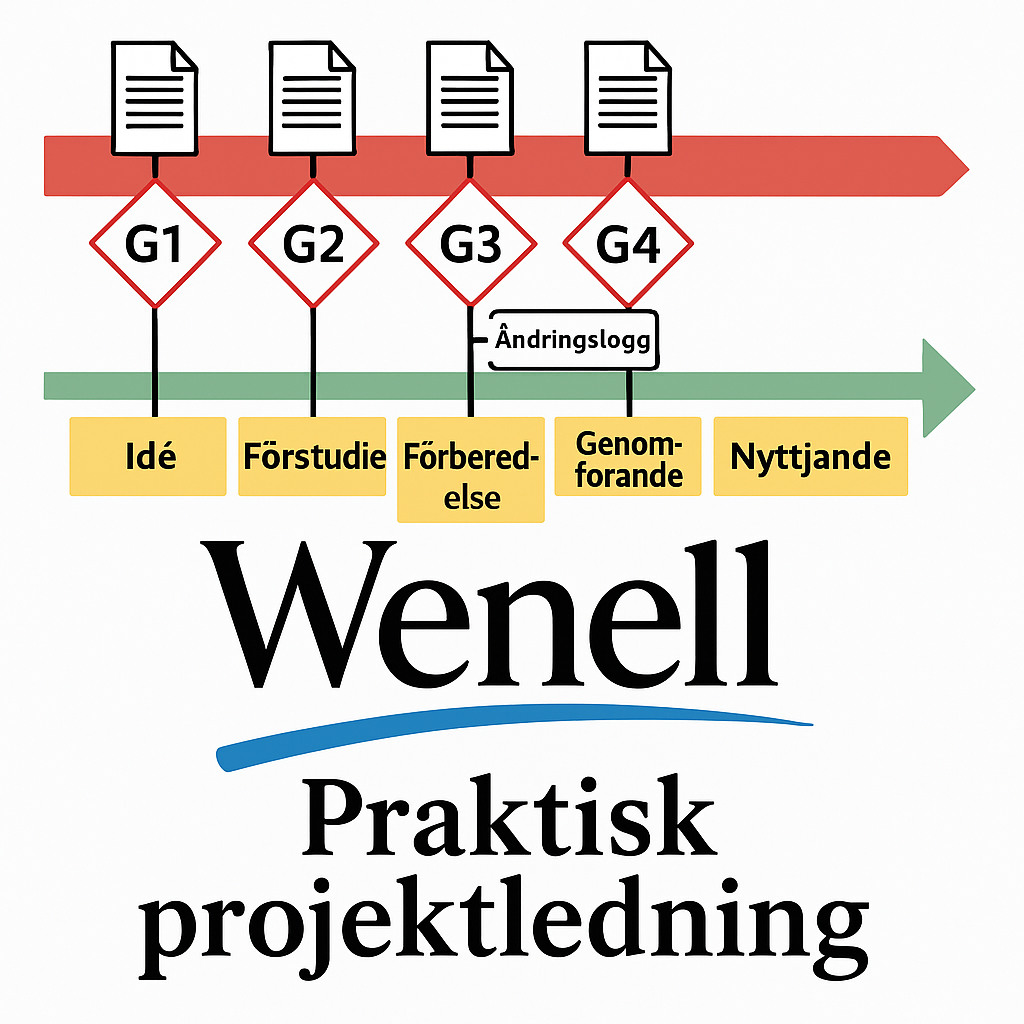
\includegraphics[width=0.9\linewidth]{../../images/wenell-ppl-badge.png}\\
%     \scriptsize Practical Project Management (Wenell)
%   \end{minipage}
%   \hfill
%   \begin{minipage}[t]{0.24\linewidth}
%     \centering
%     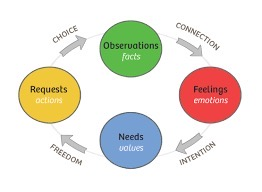
\includegraphics[width=0.9\linewidth]{../../images/nvc-year-badge.JPEG}\\
%     \scriptsize 1-Year Program in Nonviolent Communication (NVC)
%   \end{minipage}
%   \hfill
%   \begin{minipage}[t]{0.24\linewidth}
%     \centering
%     
\includegraphics[width=0.8\linewidth]{../../images/IMT_Atlantique_logo_1.png}\\
%     \scriptsize École des Mines de Nantes
%   \end{minipage}
%   \hfill
%   \begin{minipage}[t]{0.24\linewidth}
%     \centering
%     
\includegraphics[width=0.9\linewidth]{../../images/liu-logo.png}\\
%     \scriptsize Linköpings tekniska högskola (LiTH)
%   \end{minipage}
% }

% === Sections ===
%\section{Key Competencies in Projects}
{\small\ttfamily
\begin{tabular}{p{5cm} p{9cm}}
\textbf{Competency} & \textbf{Applied in} \\ \hline
Stakeholder management & Hi3G (TOM), Sony, IKEA Cloud, Nordea \\
Communication & IKEA IT (Hbg), Länsstyrelsen IT \\
Planning & IKEA IT, PUM project (diabetes), MSc thesis \\
Quality systems & Länsstyrelsen (ITIL), Nordea (PMBOK), Sony/Telenor (ISTQB), Telenor (ITIL) \\
Progress tracking & Ikano, PUM project, Bouvet (team lead) \\
Risk management & PUM project, handled operationally in Ikano/Nordea \\
Problem solving & Hi3G, Länsstyrelsen, Bouvet \\
Tight deadlines & Ikano, Telenor, Sony \\
Dynamic environment & Ikano, Nordea \\
Project evaluation & Ikano, Nordea \\
Business dev. & Not focus – delivery/stability oriented \\
\end{tabular}
}
\normalsize

%%\section{Project Management Tools}
\cvitem{Jira}{Used since 2007 when I first installed it in Cybercom’s production environment. Since then, I've used it extensively for requirement tracking, sprint planning, and Kanban workflows.}
\cvitem{Microsoft Project}{Used for creating detailed schedules, resource allocation, milestone tracking, and reporting to stakeholders.}
\cvitem{Trello}{Evaluated and introduced at Ikano as a cost-effective tool for implementing Scrum and Kanban boards, enhancing team visibility and structure.}
\cvitem{Excel / Google Sheets}{Used consistently for tracking KPIs, risk matrices, timelines, and supplementary reporting in nearly all projects.}

%\section{Ethical Hacking and PenTesting}
\cvlistitem{Nanodegree, Ethical Hacking@Udacity, Burpsuite, Kali Linux, OWASP, OSINT}
\cvlistitem{Ethical Hacking- CyberMentor@FreeCodecamp}{}
\cvlistitem{Network Fundamentals@Cisco}{}


\section{Cyber security and Cloud}
\cvlistitem{Microsoft Certified: Azure Fundamentals (AZ-900) cloud concepts, Azure core services, securituy and compliance. IaC, Powershell, Azure CLI}
\cvlistitem{Google CyberSecurity}
\cvlistdoubleitem{Red Team, Blue Team, Pink Team, Ransome Attacks, reverse-shell, HackTheBox, }{ Ethical Hacking, Miltigate Spoofing attacks, }



\clearpage
%\section{Fullstack, Frontend, Backend Development}
\cvlistdoubleitem{Client Development }  {Python, ES7+Node/javscript/typescript, React, Angular, bash/zsh,  }
\cvlistdoubleitem{Server Development, MicroServices, Java, SpringBoot/Maven} { CI/CD, Pipelines, Github/GitLab, Azure Devops}
\cvlistdoubleitem{DevOps, InfrastructureAsCode  (IoC), Docker/Kubernetes } {\{MS/My,No,Postgre\}SQL MongoDB, Redis}

%\section{Middlewware}
\cvlistdoubleitem{Low Code, Now Code, NoGo }{ Cassandra, Spark, Hive,Reddis}
\cvlistdoubleitem{SaaS, PaaS, IaaSCloud, Azure, AWS, GCP }{Bison, Powershell, Sentinel, Microsoft Defender for Cloud, Subnets,  }
\cvlistdoubleitem{System Integration, Microsoft BizTalk, (ESB) Event-Service Bus, RabbitMQ, }{Tibco Rendez-vous, Java Message Service (JMS), 
Tibco Businessworks, Tibco integration managers Scrum Master, Team Lead }


\section{Support and Application Management Experience}

\cvitem{}{
With a strong foundation in IT operations, I have extensive experience in Application Management, Problem Management, and Service Desk collaboration. At Hi3G (TRE), I acted as Application Lead for 15 critical business systems including CRM and billing, working closely with 2nd-line support and operations to ensure availability and stability.

As Problem Manager at Länsstyrelsen IT, I coordinated cross-functional teams to conduct root cause analysis, optimize support processes, and implement architectural improvements that reduced recurring errors by over 90\%. I maintained daily contact with Service Desk coordinators and domain experts across areas such as networks, GIS, hardware, and Windows infrastructure.

At Ikano Bank, I served as Release Manager and DevOps Coach, facilitating knowledge transfer, release flow automation, and coordination between development, operations, and support teams. I introduced structured deployment strategies and improved collaboration between Service Desk and backend teams.

These roles have strengthened my ability to bridge technical and user-facing domains, deliver structured problem-solving, and support users and systems with both precision and empathy.
}



%

\section{Management by Heart}
\cvlistdoubleitem{NeuroLeadership, Phychological Safety} { Neurodiversity, Trauma-informed, Inclusivity }
\cvlistdoubleitem{Agile, Lean, DevOps Culture, Safe }{PI Planning, Social Psychology, In\/out group, drama improvisation}
\cvlistdoubleitem{Trauma Therapy, PTSD litterature }{Coaching, TeamLead, Groupe Psychology}
\cvlistdoubleitem{Certified \{Tester, Scrum Master, Coach\}}{}
\cvlistdoubleitem{Consulting management, Phychology Safety} {Negotation and Prospecting, PreSales}


\cventry{Car driver's license}{}{}{}{}{}

%\cventry{Diver's license}{}{}{}{}{}

%\section{Certifications}
%\cvlistdoubleitem{Scrum Master }{ICC Coach}
%\cvlistdoubleitem{ISEB / ISTQB  (Test)}{React nanodegree }

\section{Developer Experience (Support-Oriented)}

\cventry{2017--2018}{Verisure Innovation}{Senior Software Engineer}{Malmö}{Java, Android, Kubernetes}{
Contributed to internal IT tools for camera installers and support teams. Led GDPR compliance integration and worked cross-functionally with legal and infrastructure teams to ensure user data protection. Designed a deployment pipeline to improve reliability and reduce downtime for support-critical systems.
}

\cventry{2015--2016}{Länsstyrelsernas IT-enhet}{Problem Manager}{Remote}{ITIL, Incident/Problem mgmt}{
Led problem-solving across departments including Service Desk, GIS, Network and Print. Reduced critical error codes from 1400 to 50 per month. Introduced structured follow-ups, escalation workflows and architectural fixes to prevent recurring incidents.
}

\cventry{2012--2014}{IKANO Bank}{Release Manager / DevOps Coach}{Remote}{.NET, BizTalk, Jenkins}{
Managed application deployments and cross-team coordination. Acted as a liaison between operations, support and developers. Automated release processes and improved documentation, reducing support effort and handover confusion. Collaborated actively with Service Desk during handovers.
}

\cventry{2011--}{Hi3G (TRE)}{System Integration Specialist \& App Lead}{Stockholm}{TIBCO, CRM Integration}{
Owned application landscape integration for 15 systems. Supported CRM and billing platforms, with close contact with Service Desk and infrastructure. Provided 2nd-line support, coordinated incident resolution and ensured system availability during critical operations.
}

\cventry{2008--2010}{IKEA IT}{Project Coordinator \& Support Tools Rollout}{Helsingborg}{Java, PCI DSS}{
Coordinated rollout of custom IT tools to bridge in-store operations and central IT. Ensured usability and technical stability of internal support systems. Collaborated with store staff, support agents, and infrastructure teams.
}

\cventry{2004--2012}{Telenor}{Integration Specialist}{Oslo/Malmö}{Java EE, Tibco, BPM}{
Contributed to integration testing, Jira plugin development, and architecture documentation. Worked closely with business units and operations to ensure stable middleware performance. Support-focused development with emphasis on maintainability.
}


\section{Technical Skills}

\cvitem{}{%
\textbf{Operating Systems:} \\
Windows 10/11, Windows Server, macOS, Ubuntu/Linux
}

\cvitem{}{%
\textbf{Support Tools \& Service Platforms:} \\
Microsoft Service Desk, Remedy, Jira, Confluence
}

\cvitem{}{%
\textbf{Cloud \& Scripting:} \\
Microsoft Azure (AZ-900), PowerShell, Azure CLI, Python
}

\cvitem{}{%
\textbf{Network \& Troubleshooting:} \\
DNS, TCP/IP, VPN, Remote Desktop, printer \& hardware diagnostics
}

\cvitem{}{%
\textbf{Office \& Collaboration:} \\
Microsoft 365, Teams, SharePoint, Outlook
}

\cvitem{}{%
\textbf{IT Methodologies:} \\
ITIL, Incident \& Problem Management, Documentation \& Root Cause Analysis
}




\section{Education}

\cventry{1996--2003}{MSc in Computer Science and Engineering}{Linköping Institute of Technology}{Linköping}{}{}

\includegraphics[scale=0.4]{../../images/it-security}
\cventry{2016}{Python Programming \& Problem Solving (2.5 ECTS)}{Blekinge Institute of Technology}{Ronneby}{}{}

\cventry{2023--2024}{CyberSecurity Fundamentals}{Google / Coursera}{Online}{}{}

\cventry{2022--Ongoing}{Cloud \& DevOps Labs}{Udacity}{Remote}{Grafana, Terraform, Kubernetes, AWS}{}

\cventry{2023--Ongoing}{Public Speaking \& Communication}{Toastmasters}{Lund}{}{}

\section{Education}
\cventry{2023 HT-- 2024 VT}{Google CyberSecurity Fundamentals}{Google/Coursera}{ }{}{} 
\cventry{2023 VT -- Ongoing}{ToastMasters}{Lund}{ }{Public Speaking}{} 
\cventry{2022 HT -- Ongoing}{SRE, Fullstack and Front-end}{Udacity@Palo Alto}{ }{Grafana, Terraform, Kubernetes, AWS}{} 
\cventry{2020}{Pedagogical Drama, Story Telling, Improvisational theatre, Groupe Dynamics}{Malmö University}{Malmö}{}{}      
\cventry{2019-2021}{React.JS (ES6, React, Router, Redux, Native) Nanodegree}{Udacity@Palo Alto}{Remote}{}{}  
\cventry{2016}{Programming and Problem-solving in Python. 2.5 ECTS}{Blekinge Institute of Technology}{Ronneby}{}{}  
\cventry{1996 --2003}{MSc in Computer Science and Engineering. 300 ECTS}{Linköping Institute of Technology}{Linköping}{}{Computer/IT-Security, Software production, Artificial Intelligence, Object-Oriented Programming, Functional Programming, Real time programing, Lisp/C, Advanced computer architecture, Hardware construction, Embedded development with micro-controller}  

\section{Certifications \& Additional Training}
\cvitem{Microsoft Azure}{Certified Azure Fundamentals (AZ-900)}
\cvitem{Agile \& Scrum}{Certified Scrum Master (CSM), Softhouse}
\cvitem{IT Service Management}{ITIL Foundation (internal knowledge)}
\cvitem{DevOps Tooling}{CA Lisa/Nolio – Continuous Delivery Automation}
\cvitem{Communication}{18-day Nonviolent Communication (NVC) Program}
\cvitem{Coaching}{ICC Certified Coach – SLH, Thailand}

% \section{Master thesis}
% \cvitem{Title}{\emph{On the automatic evolution of an OS kernel using temporal Logic and AOP}}
% \cvitem{Supervisors}{Julia Lawall phD, Mario Südholt phD, Gilles Muller phD}
% \cvitem{Description}{
% In IEEE International Conference on Automated Software Engineering, Montréal, Canada, pages 196 --204, 42 citations}
% \url{https://www.researchgate.net/publication/220883611\_On_the_automatic_evolution_of_an_OS_kernel_using_temporal_logic_and_AOP}



\section{Testimonials}

{\small
\begin{quotelist}
  \item \textit{``Rickard became rapidly proficient in all technologies by effectively communicating with the research engineers and has delivered to all my requirements.''} \\
  — Mario Südholt, Associate Professor, OBASCO Group, École des Mines

  \item \textit{``Rickard has rapidly, with great accuracy and interest fulfilled the requirements of which the roles demanded. He is also responsible and enterprising.''} \\
  \textit{``Rickard’s work has meant close cooperation with several clients and demanded great communication skills to understand the end-users needs. We give him our best recommendations.''} \\
  — Cybercom

  \item \textit{``Rickard is ambitious and dedicated to his work and his team – the reason for our success with a stable environment.''} \\
  — Frank Amersbasch, Head of Technical Operations, Ikano Bank

  \item \textit{``Rickard has not only used the existing processes but also simplified and improved them. Rickard is goal-oriented, planning-oriented and flexible.''} \\
  — Jonas Paulsson, Länsstyrelsen IT
\end{quotelist}
}



%
\large
\section {Project Mgmt, Scrum master etc}
\cventry
  {Maj 2025–}
  {Driving force in Wellness Startup project + HRV}
  {@ RMTS for Depression, Malmö}
  {} % empty date/location row
  {}
  {Help patients manage stress and wellness to relieve anxiety, depression, chronic stress, and insomnia. 
  Expert on HRV, VNS and signal processing (DFT, FFT, Arduino, DAC). Agile project management using Kanban and Trello.}

\cventry
   {2020–2025}
  {Trauma-Informed Group Facilitator, ACOA}
  {@ Online (Zoom)}
  {}
  {}
  {Facilitated Zoom-based peer-support meetings for Adult Children of Alcoholics (ACOA), using trauma-informed leadership rooted in principles from Internal Family Systems (IFS) and Nonviolent Communication (NVC). Held space for vulnerable sharing, emotional regulation, and mutual trust. Responsibilities included timekeeping, check-ins ("presentation and how do you feel"), group decision-making (group conscience), and facilitation of structured material such as *The Red Book* and *The Loving Parent Guidebook*. Developed transferable skills in psychological safety, presence-based leadership, and deep listening — directly applicable to Scrum Master and project leadership roles in high-trust IT environments.}

\cventry
  {2017–2018}
  {Sub Project Manager, GDPR Compliance}
  {@ Verisure}
  {}
  {}
  {Managed a GDPR compliance sub-project focused on internal employee-facing applications. Coordinated cross-functional efforts to ensure data privacy, consent handling, and secure processing of personal information. Worked closely with legal, IT, and product teams to align backend systems with new regulatory requirements. Delivered updated app modules supporting data subject rights and transparency in line with GDPR.}

% \cventry{2015-2016}{Problem Manager}{@ Länsstyrelsernas IT-enhet}{}{}{ITIL, problem process, incident management, service management, cross-functional teams, root cause 
% }  

% In the role as Problem Manager within Länsstyrelsernas IT-enhet, via Västra Götalands region I have driven, and coordinated meetings to solve problems spanning over different departments. Daily contact with incident managers, the coordinator for service desk, service managers for areas such as Webb, Network, Print, Hardware, Gis, Windows, Integration and message technology. Identifying bottlenecks in groups, and roles and escalating to process owner and senior management. Successfully implemented a new architecture together with an architect in one area which decreased monthly error codes from 1400 to 50.  

% \cventry{2014-2015}{Senior Project Manager / Scrum Master}{@ Nordea}{Cph/Denmark}{}{Several roles, Scrum, DevOps, Java }  
% In the role as DevOps Coach / Scrum master I have introduced agile/scrum methodologies and tools (git, jira, confluence) for a cross-functional team consisting of Operation Specialist, Automic specialists and Developers to setup test environments (preprod/uat), deployment, alarms and monitoring solutions. 

% Facilitated Scrum artefacts such as: 
% \begin{itemize}
%     \item Sprint planning meetings 
%     \item Sprint Demo 
%     \item Retrospective 
%     \item Individual coaching sessions 
% \end{itemize}

% In the role as Senior Project Manager I’ve been driving different infrastructure projects around IaaS/Amazon EC2 PoC: 
% \begin{itemize}
%     \item Project planning and documentation 
%     \item Setting up QRA – risk analysis  
%     \item Started a cross organizational local group for puppet automation, to share knowledge.
%     \item Contact with vendors, AWS and Tibco for Staffing and advise 
%     \item Initial architecture for grid solution based on Tibco DataSynapse, and Amazon EC2 for a computing grid in the cload. 
%     \item Hands-on java coding to interface to an integration motor, to provide a framework for an improved deployment solution. Springboot, maven3,  
% \end{itemize}


% \cventry{2012-2014 }{DevOps, Automatic Deployment, Knowledge Transfer, Release Management }{@ IKANO Bank}{}{}{desc}  
% \begin{itemize}
%     \item I was responsible and secured the deployment of ikanobank.se. One part of the project was to faciliate a knowledge-transfer from Germany to Denmark. At the same time I took several initatiatives necessary to create a succesful environment to deploy in, both technical-wise and process-wise. 
    
%     \item The continuous improvements, knowledge-transfer, documentation clean-up, retrospectives, coaching of ops team in agile methods and introduction of ways of working with a DevOps/C.D. Tool, CA Lisa resulted in decreased resources by about 75\% and improved quality multiple times. Handling and took initiatives to several sub-projects. 
    
%     \item Technology stack: MS .NET, BizTalk, CA Lisa/Nolio, Jenkins, Infrastructure, Load balancing, SCOM etc. Led a team of operations specialist and coordinated work between 15 people including developers, testers, etc. 
    
%     \item Work in Germany, Denmark and Sweden. 
% \end{itemize}
\cventry{2014--2015}{Senior Project Manager \& Scrum Master}{Nordea}{Copenhagen}{Scrum, DevOps, Java}{
\textbf{DevOps Coach:} Introduced agile methods (Scrum, Kanban), Git, Jira, and Confluence in a cross-functional team (Operations, Automic, Development). \\
\textbf{Scrum Facilitation:} Led sprint planning, demos, retrospectives, and coaching sessions. \\
\textbf{Infrastructure Projects:} Managed IaaS/Amazon EC2 PoC, performed risk analysis (QRA), initiated Puppet automation group. \\
\textbf{Architecture \& Coding:} Designed grid solution with Tibco DataSynapse and EC2; developed Spring Boot-based deployment integration prototype.
}

\cventry{2012--2014}{DevOps Lead \& Release Manager}{IKANO Bank}{}{.NET, BizTalk, Jenkins, Nolio}{
Led deployment of \texttt{ikanobank.se}, bridging technical and process needs. \\
Facilitated knowledge transfer from Germany to Denmark and introduced automated deployment via CA Lisa/Nolio. \\
Improved quality and efficiency through documentation cleanup, agile coaching, retrospectives, and team coordination (15+ people). \\
Worked across Sweden, Denmark, and Germany.
}

\cventry
  {2008–2009}
  {Project Coordinator, Custom Worktop Rollout}
  {@ IKEA IT}
  {}
  {}
  {Coordinated the rollout of a customized IT support system for made-to-measure kitchen worktops across multiple countries. Managed requirements gathering, project timelines, acceptance testing, and user onboarding. Bridged central IT systems with in-store operations for smooth implementation.}

\cventry
  {2005–2007}
  {Test Manager, R2R Program (Sony Ericsson)}
  {@ Sony}
  {}
  {}
  {Led the test efforts for two sub-projects within the global Record-to-Report (R2R) transformation program. Responsible for test strategy, planning, test cases, and defect management. Worked cross-functionally with development and business teams to ensure quality in financial processes and reporting systems.}



\section{Employments}
\cventry{2025}{Cloud Computing och Azure-kurs}{ReDI School of Digital Integration}{}{}{
Praktisk kursfokuserad utbildning inom Azure, molnsäkerhet och DevOps. Förberedelse inför certifiering med case-baserade projekt.
}
\cventry{2021-12 -- 2022-06-01 }{ADBSafegate AB}{ADBSafegate AB}{Malmö}{Fullstack Developer}{Angular, typescript, Azure, Scaled Agile Framework, SAFe}
\cventry{2021-06 -- 2021-09 }{Zaplox AB}{Zaplox AB}{Lund}{Fullstack Developer}{Vue.js node javascript css AWS}
\cventry{2019-2021 }{React.JS Nanodegree}{Udacity}{Remote}{}{Portfolio Projects - reviewed and passed by react experts}
\cventry{Aug 2017-Nov 2018}{Senior Software Engineer}{Verisure Innovation}{Malmö}{}{}
\cventry{May2012 -- Dec2017}{Managing Consultant}{Bouvet Syd AB}{Malmö}{}{Java Developer, Team Leader/CUManager/Partner Responsible DevOps}
\cventry{May2004 --Feb 2012}{Consultant}{Cybercom}{Malmö}{}{Java, Integration, Test}
 \cventry{Mar 2003 --Feb 2004}{RnD Engineer}{Ecole Des Mines}{Nantes/France}{}{}
\cventry{Mar 2003 --Feb 2004}{Thésard}{Ecole Des Mines}{Nantes/France}{}{MSc Thesis}
\cventry{Jul 2002 -- Sep 2002}{Embedded Developer}{Hemocue}{Ängelholm}{}{}

% \section{Interests}
% \cvitem{hobby 1}{Yoga and Meditation}
% \cvitem{hobby 2}{Dance and Martial Arts}
% \cvitem{hobby 3}{Singing and playing piano}

\section{References}
Lämnas på begäran.



% \nocite{*}}

% \bibliographystyle{plain}
% \bibliography{publications}                        % 'publications' is the name of a BibTeX file

\clearpage
\Large

\end{document}  